%!TEX ROOT = thesis.tex
\chapter{Framework Overview}
\label{chapter:framework}
\section{Introduction}
To tackle the issues identified through the research questions and literature review, a theoretical framework is first laid out to provide a conceptual schema to break the intricate problem into multiple sub-tasks. Firstly, the overview of the proposed framework used in this work is described in Section \ref{section:framework}. Next, the description of the dataset used is given in Section \ref{section:dataset_used} and finally, this chapter concludes with the experimental methodology applied to obtain the results (presented in Section \ref{sec:expmethodology}).


\section{Framework Overview}
\label{section:framework}
In this section, a high-level overview of the fundamental processes along with two suggested core components for vehicle semantic extraction and retrieval is provided.
The groundwork described in this work abides by the typical top-down approach used in Intelligent Transportation System (ITS) where the video data is subjected to background subtraction, followed by blob filtering, vehicle detection as well as vehicle tracking, as thoroughly described in \cite{lim2017}.
The semantic information of the vehicle blobs are then extracted and stored in the database.

Now, with the vehicle-specific semantics stored in the database, retrieval engines are designed to enable users to easily retrieve the stored information. The retrieval engines feature a graphical user interface (GUI) that allow users to enter the queries by drawing the desired trajectory on the search interface and provide other crucial information which would assist in identifying the targeted video sub-sequence or \emph{shot}.

However, as mentioned in the scope of thesis (Section \ref{subsec:scope}), the bounding box of the vehicles are assumed to have been obtained prior to the semantic extraction task. Hence, the semantic extraction and video retrieval processes are the central emphasis of this thesis.

\begin{figure}[hbt!]\centering
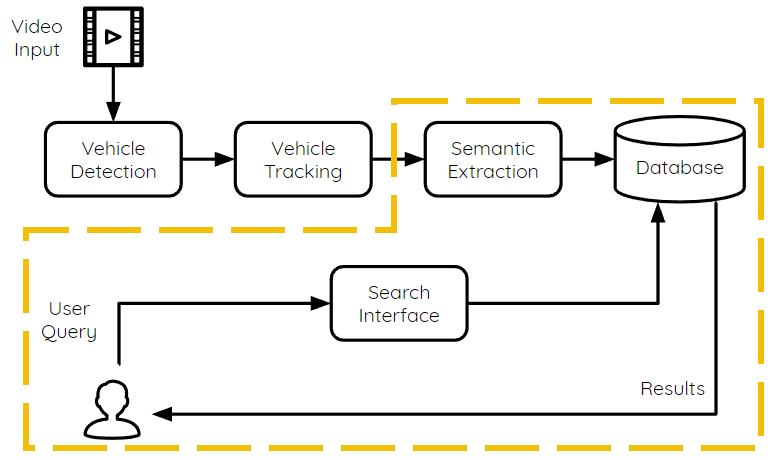
\includegraphics[width=.9\textwidth]{image/new/framework_new.PNG}
\caption{Framework Diagram. Contribution Highlighted in Area Marked with Yellow Dashed Borders.}
\label{fig:framework}
\end{figure}

In this thesis, a framework is suggested and used for the vehicle semantic extraction and vehicle semantic retrieval tasks.
The proposed methods were developed in two cascading phases (see Figure ~\ref{fig:proposedmethodoverview}) with the same corresponding objective for each task.
The formulation of the idea, steps and processes involved in each phase is described in this chapter.
On a whole, the end-to-end framework can be visualised using Figure ~\ref{fig:framework} where the main contribution of this thesis is highlighted with a yellow dashed border.

\subsection{Phase 1: LSH-Inspired Semantic Extraction and Retrieval Technique}
\label{subsec:lsh-intro}
The first of the two techniques suggested in this thesis is the \textit{LSH-Inspired Semantic Extraction and Retrieval Technique}. Locality-Sensitive Hashing (LSH) as introduced by~\citeA{indyk1998approximate} was originally used for devising main memory algorithms for nearest neighbor search. This technique was later used by~\citeA{kulis2009kernelized} to embed high-dimensional features from images into low-dimensional Hamming space (dimensionality reduction) where items can be efficiently search. 
Unlike conventional hashing techniques that aims to avoid hash collisions, LSH tries to maximise these hash collisions. When performed on a set of documents, documents with similar properties are mapped and clustered to a similar locality or neighbourhood. This technique excels especially when working with high dimensional data such as video data.
%However, the exact implementation of LSH is not employed in this work. Instead, 
We draw inspiration from LSH on how similar ``documents'' can be clustered. %and implemented in this phase. 
The extracted semantics from each vehicle blobs were clustered into semantic groups consisting of 11 colours and 9 motion clusters. This concept is adopted in the proposed method with the following considerations in mind:
\begin{enumerate}
    \item Easing Interpretation \& Access: As the extracted semantics are stored in clusters of similar properties, these semantics can be easily interpreted and retrieved when required.
    \item Easing Input/Output (I/O) Bottleneck: As the proposed method stores the extracted semantics in a database, I/O bottlenecks are bound to occur when reading and retrieving large quantities of data. Given that semantics of similar properties were clustered together, the retrieval technique only has to search through these identified semantic clusters in an efficient manner instead of the entire database for matching records.
\end{enumerate}


\subsection{Phase 2: CD-Inspired Semantic Extraction and Retrieval Technique}
The second technique suggested in this thesis is the \textit{Chamfer Distance-Inspired Semantic Extraction and Retrieval Technique}.
Chamfer Distance (CD) is one of the many distance measures %(see Section \ref{section:distancemeasures})
introduced by mathematicians and researchers. Chamfer Distance, as introduced by~\citeA{barrow1977parametric}, was originally designed to match images by comparing the shapes of two collections of shape fragments.
However, in this thesis, the use of CD was adapted to suit the research problem of comparing vehicle trajectories' shapes. While the implementation of CD measure in this framework has its advantages, it also comes with certain drawbacks. The considerations taken when designing this technique is as follows:
\begin{enumerate}
    \item The use of Chamfer Distance to compare trajectories allows the retrieval technique to search from a wider range. While this comes with additional computational costs which are undesirable, the increased in robustness outweighs the drawbacks. Along with that, effective time and date filtering could potentially reduce the number of records, hence, further reducing the computational cost.
    \item Effective ranking of results is a desirable characteristic in any retrieval engine. As Chamfer Distance produces a distance score for every pair of trajectories compared, this score can be used to sort the results in an intuitive manner where results of higher similarity or resemblance would appear higher in the ranked retrieval results.
\end{enumerate}


\section{Dataset}
\label{section:dataset_used}

In view of testing the proposed framework, a new video dataset was gathered as there are limited long-term outdoor car park datasets that are publicly available for research. A stationary cloud-enabled web camera was set up in a room (with a glass window) on the fourth floor of a building facing a relatively large outdoor car park area. Figure \ref{fig:camerasetup} illustrates the location of the camera that was set up to overlook the adjacent car park area.
%The aforementioned setup was done to mimic a typical camera setup which towers over a piece of outdoor car park lot that is found in the wild.
\begin{figure}[hbt!]\centering
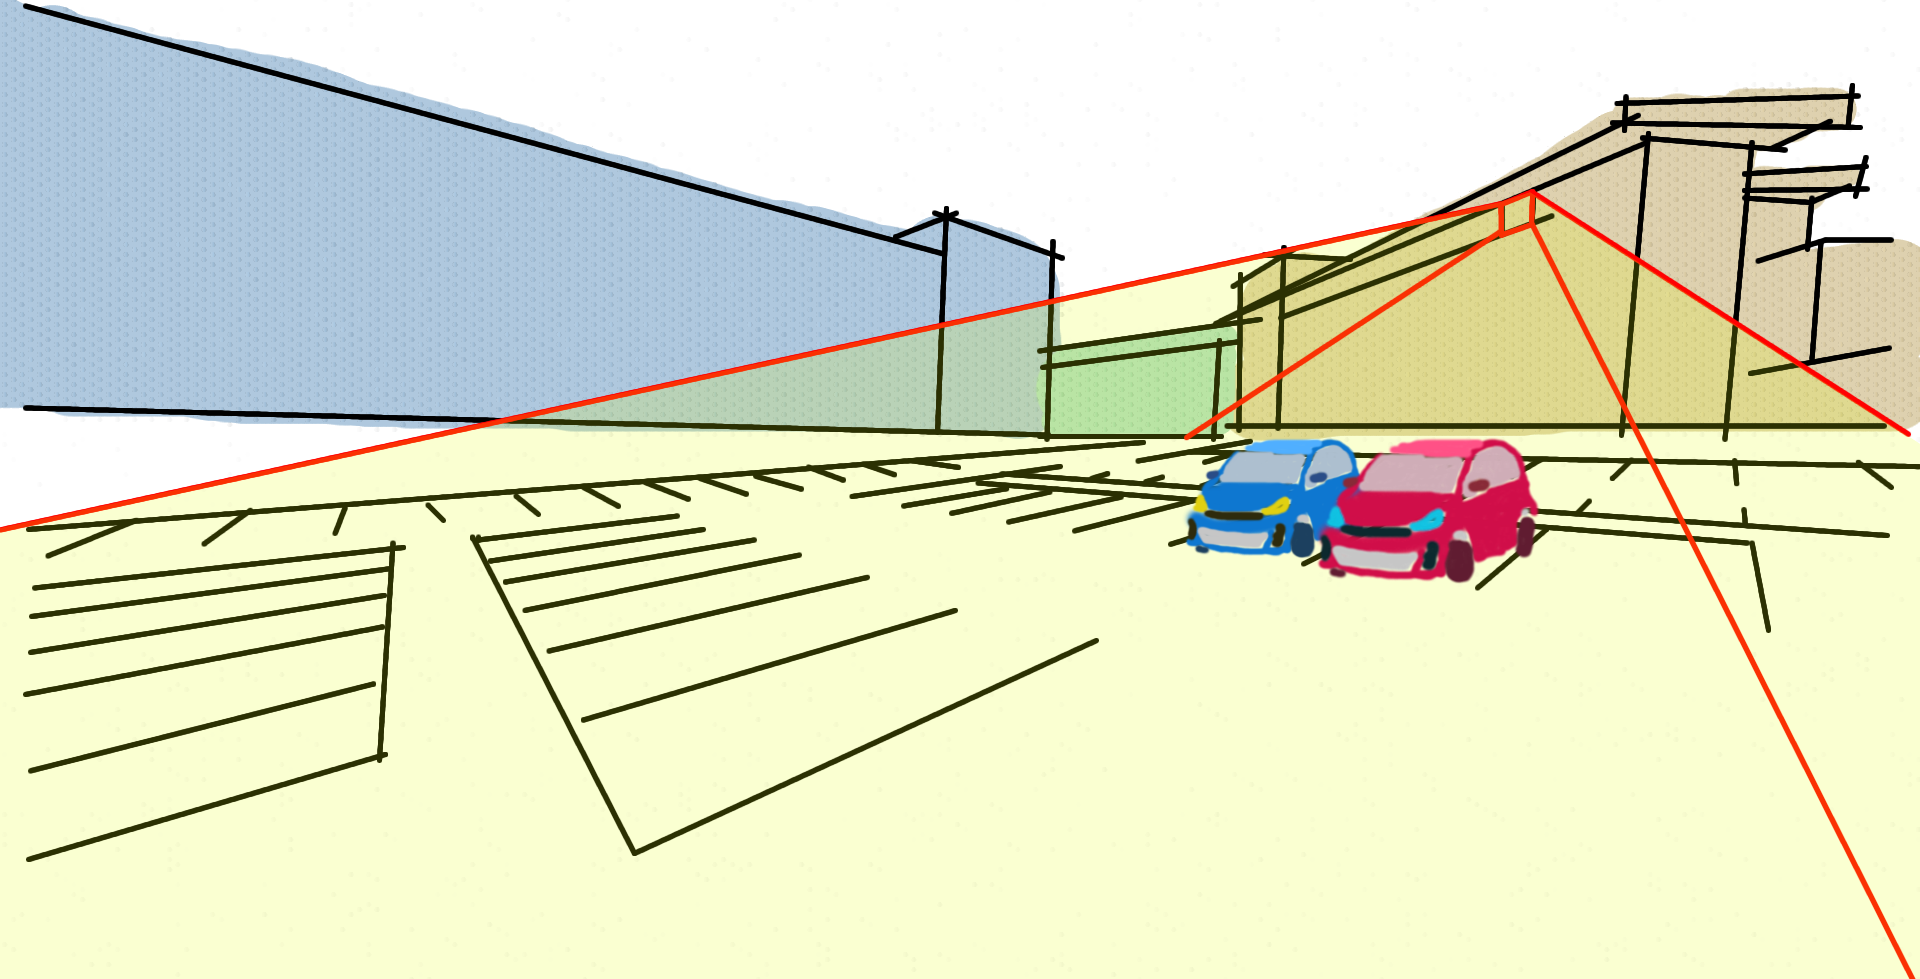
\includegraphics[width=.8\textwidth]{image/new/fcicarpark2.png}
\caption{Camera Setup to Capture the Car Park From the Fourth Floor}
\label{fig:camerasetup}
\end{figure}
\begin{figure}[!hbt]\centering
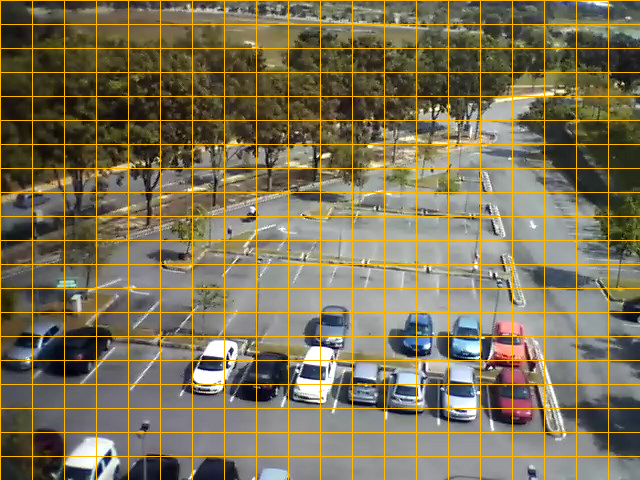
\includegraphics[width=.7\textwidth]{image/general/grids.png}
\caption{View From Camera Setup; 20$\times$20 Grids}
\label{fig:viewfromcamera}
\end{figure}

Through the camera's web interface, the device was set to record on weekdays from Monday through Friday, starting from 08:30 up until 18:30 in the evening, totaling 10 hours of video recorded each day. To obtain smaller file sizes, each recorded video clip was set to have a maximum length of 6 minutes, hence a total of 100 videos were obtained at the end of each day. The recorded video clips were then stored in a microSD memory card.
At the end of each day, the data was copied over to a server via a script. However, due to a few sporadic glitches that occurred during the recording process, some of the video clips had missing portions. Hence, some of the days did not contain the full 10 hours of video clips.

\begin{table}[!ht]\centering
\begin{tabular}{|l|l|}
\hline
Camera Model & Dlink DSC-942L        \\
Resolution   & 640$\times$480 pixels \\
Frame rate   & 10 $fps$             \\
Format       & H.264 / MPEG-4 AVC    \\
Naming Convention & $CCYYMMDD\_HHMMSS.mp4$ \\
\hline
\end{tabular}
\caption{Details of the Camera Setup used for Data Collection}
\end{table}

\begin{figure}[!htb]
  \centering
  \begin{tabular}{cc}
 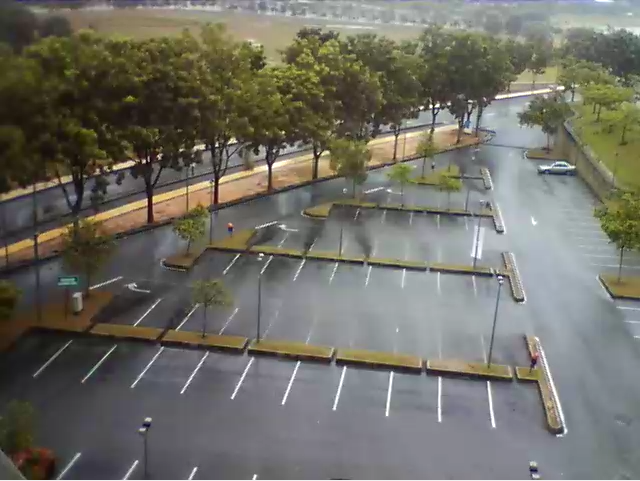
\includegraphics[width=0.4\linewidth]{image/general/rain.PNG} &  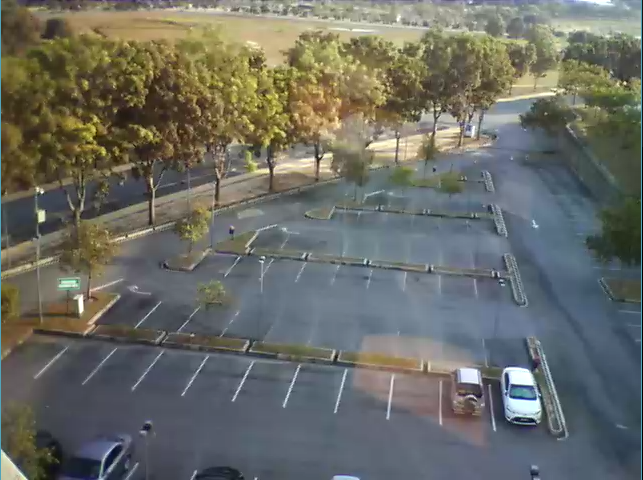
\includegraphics[width=0.4\linewidth]{image/general/reflection.PNG}\\
\begin{tabular}{c}(a) Rainy day with \\ reflective surface\end{tabular} & \begin{tabular}{c}(b) Reflection on the \\car park from the window\end{tabular} \\
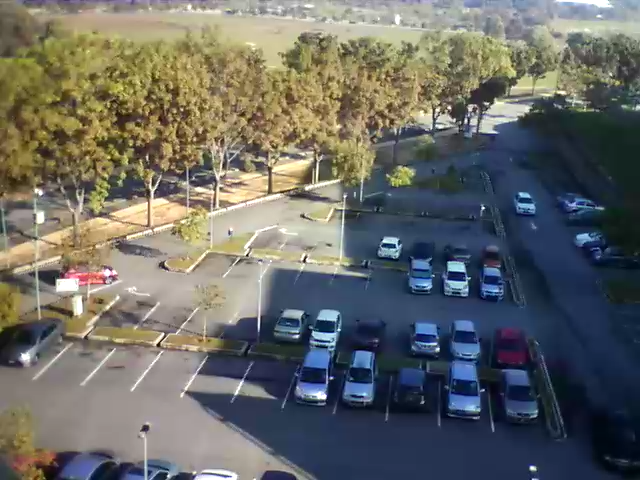
\includegraphics[width=0.4\linewidth]{image/general/shadow.png} &  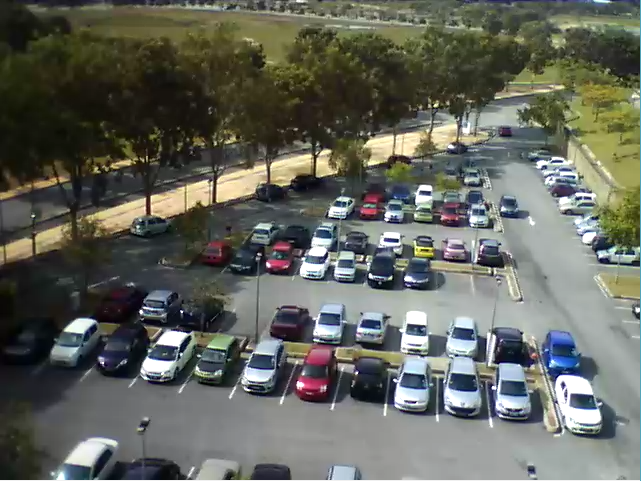
\includegraphics[width=0.4\linewidth]{image/general/shadow2.png}\\
\begin{tabular}{c}(c) Severe shadow over \\ the car park (08:48AM)\end{tabular} & \begin{tabular}{c}(d)  Severe shadow over \\ the car park (04:06PM)\end{tabular}
\end{tabular}


\caption{Noisy Data Within the Collected Dataset} \label{fig:weather}
\end{figure}

This data acquisition setup was left to record data over the course of several months under various natural weather and lighting conditions. This also includes a diverse set of car park scenes such as peak hours with plenty of vehicles along with the off days. Along with that, this setup covers a total of over 45 parking lots excluding parking lots that are too small or occluded. Figure \ref{fig:weather} illustrates the various weather conditions and noise which were recorded sporadically throughout the dataset.


\section{Experimental Methodology}
\label{sec:expmethodology}

In the subsequent chapters, the detailed descriptions of the proposed vehicle semantic extraction algorithm as well as the retrieval techniques will be provided. This section briefly describes the methodology and the experimental setup to provide an overview of how the experiments were performed in this thesis.

As the performance of the proposed methods is essential towards end-users, each of the proposed algorithm in the framework was evaluated with the help of volunteers.
The bounding box obtained using the Vehicle Detection and Vehicle Tracking framework proposed by \cite{lim2017} included errors. While these errors were propagated to the Vehicle Semantics Extraction and Retrieval modules, they were not overlooked nor discarded during the evaluation process. This was done intentionally to provide an end-to-end assessment of the framework.

The proposed methods were implemented and evaluated on an Intel i7 machine with 16GB RAM, equipped with a GeForce GTX 1060 GPU. As the main focus of the proposed method revolves around the semantic extraction and retrieval of \textbf{vehicle colour} along with the \textbf{vehicle trajectory}, both of these components were assessed and evaluated individually.
This was done to better understand the performance, effectiveness as well as the weakness of the proposed methods.

As a result, two different phases were introduced to enhance the performance based on the obtained intel and gaps which were identified via experimental results. This also allowed us to gain a deeper understanding of the proposed method along with the opportunities for future improvements.
Likewise, the experimental methodology can be divided into two phases.
%Two retrieval techniques were designed and implemented in this work, the objective of the first retrieval engine was to build a prototype for the evaluation of its current performance and to identify gaps to be improved. This process allowed the author to return to the drawing board and reevaluate the algorithms, metrics and evaluation process performed.


\subsection{Phase 1: LSH-Inspired Semantic Extraction and Retrieval Technique (Prototyping)}
While the collected dataset comprised of several months of data, only two days of data (20 hours) were used for the evaluation of \versionOneRet. Several annotators were deployed to manually label and fully annotate these data. Upon completing the annotation process, the annotators would cross-check to verify the sanctity of the annotation.
Along with that, the cross-checking allows the annotators to arrive at consensus on annotations that did not tally. The annotators were asked to take note of the following events:
1) Number of vehicle of each colour category (11 categories, see Table~\ref{table:colorshex}), and 2) Number of vehicles performing motion $TQ1$ \& $TQ2$ (See Figure \ref{fig:versionOneInterface}).
Having fully annotated data allowed us to evaluate the performance of the proposed method using the Accuracy, Recall and $F_1$ Score metrics.

\subsection{Phase 2: CD-Inspired Semantic Extraction and Retrieval Technique (Full Experiment)}

During the \textbf{Phase 1} experiment, it was noted that the entire annotation process took a significant amount of work despite only using two days of data. As one month of data was set aside for the evaluation of the \versionTwoRet, an alternative experimental methodology was applied.
Typical with any large-scale retrieval engine of all intents and purposes, it is not feasible to annotate a huge amount of ground truth manually as it takes an enormous effort which is time-consuming.
Hence in \textbf{Phase 2}, semantics from one month of data was extracted, retrieved and evaluated without the manual annotations of any events.

As the final output of this proposed method is an end-user facing retrieval system, the evaluation process took on an empirical user study approach. This unbiased approach provided the volunteers with full control and freedom to perform any kinds of query over the search interface.
Using this setup, a group of six volunteers were performed a total of 11 queries on the retrieval engine for both the vehicle colour and trajectory semantics.
%of the vehicles and provide relevance score for each retrieved results.
Based on each query, the volunteers were tasked to provide relevance score($REL$) and evaluation for each of the randomly ordered retrieved results.
As the data in this phase was not fully annotated, it is impossible to compute the Recall and $F_1$ score. Instead, the Precision@K along with the normalised Discounted Cumulative Gain (nDCG) metrics were used.

